\subsubsection{Основной алгоритм}
В ходе разарботки был применен видоизменнённый шаблон проектирования Factory method.

%Описание шаблона и его модификации
Данный шаблон относится к классу порождающих шаблонов. Шаблоны данного класса - это шаблоны проектирования, которые абстрагируют процесс инстанцирования (создания экземпляра класса). Они позволяют сделать систему независимой от способа создания, композиции и представления объектов. Шаблон, порождающий классы, использует наследование, чтобы изменять инстанцируемый класс, а шаблон, порождающий объекты, делегирует инстанцирование другому объекту.
Пример организации проекта при использовании шаблона проектирования Factory method представлен на рисунке \ref{architech:architech}.

\begin{figure}[h!]
\center{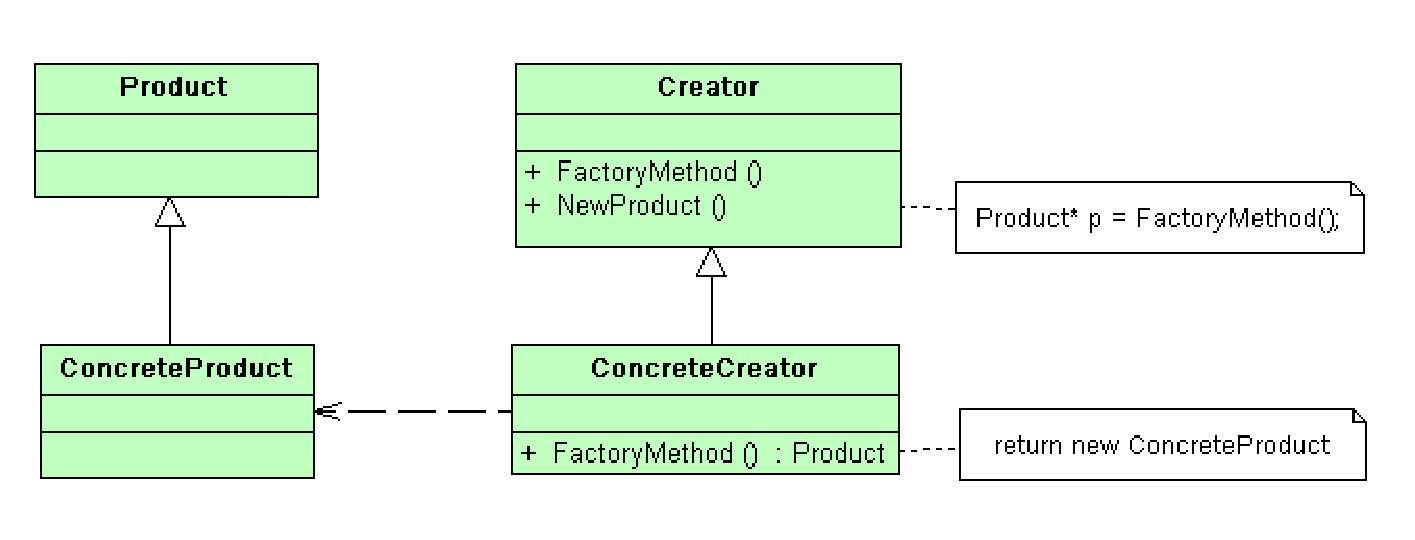
\includegraphics[width=0.9\linewidth]{architech}}
\caption{Пример организации проекта при использовании шаблона проектирования Factory method}
\label{architech:architech}
\end{figure}

Использование данного шаблона позволило разбить проект на независимые модули, что весьма упростило задачу разработки, так как написание алгоритма для конкретного таска не влияло на остальную часть проекта. При разработке был реализован базовый класс для работы с образом диска. Данный клас предназначался для формирования списка настроек, определения операционной системы на смонтированном образе и инстанционировании и накапливание всех необходимых классов-тасков в очереди тасков. После чего каждый таск из очереди отправлялся на выполнение. Блоксхема работы алгоритма представлена на рисунке \ref{alg_main:alg_main}.

\begin{figure}[h!]
\center{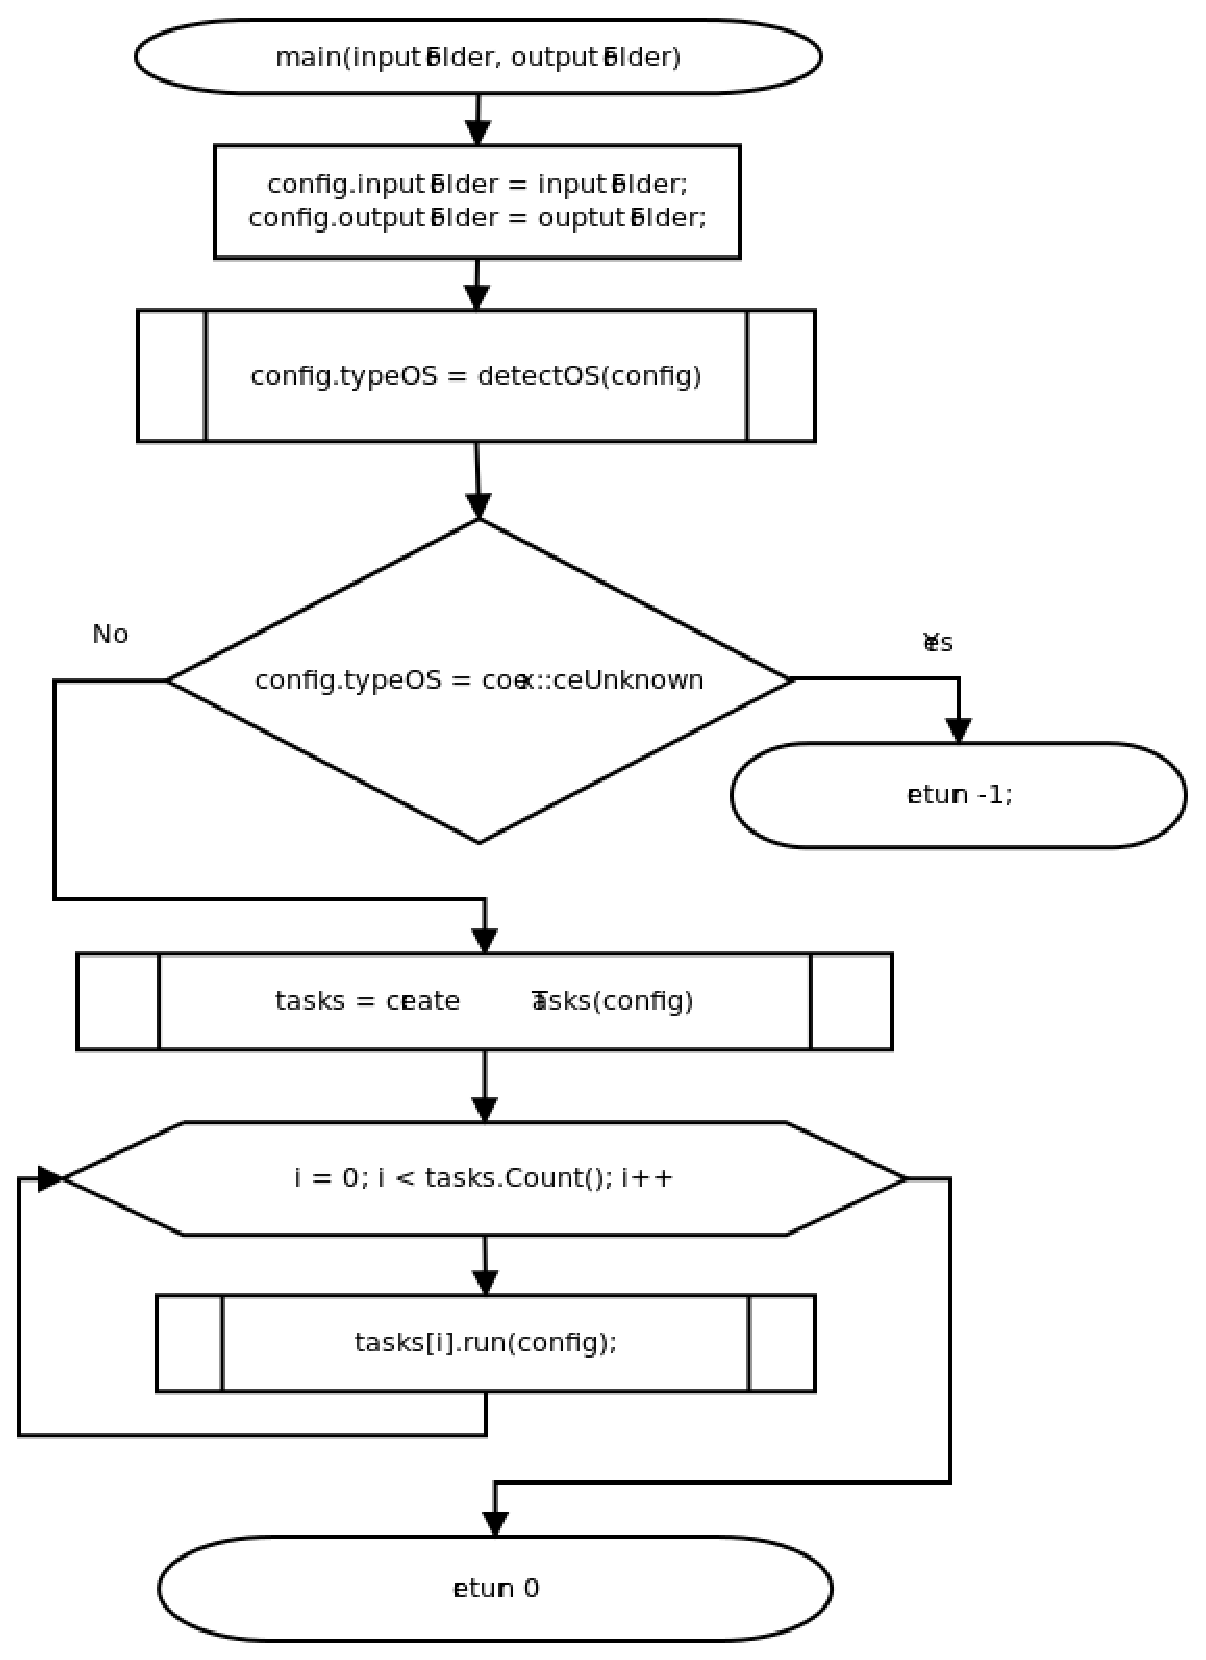
\includegraphics[width=0.6\linewidth]{alg_main}}
\caption{Алгоритм работы с образом диска}
\label{alg_main:alg_main}
\end{figure}

Каждый класс-таск порождался путем наследования от базового абстрактного класса который имеет 8 методов и 3 атрибута:

\begin{enumerate}
\item QString manual() - возвращает справку о входных параметрах данного таска;
\item void setOption(QStringList list) - установка флагов для поданных на вход параметров;
\item QString command() - возвращает команду для инициализации таска вручную;
\item bool supportOS(const coex::typeOS \&os) - возвращает флаг, указывающий на возможность использования данного таска для конкретной операционной системы;
\item QString name() - возвращает имя данного таска;
\item QString description() - возвращает краткое описание таска;
\item bool test() - предназначена для теста на доступность таска;
\item bool execute(const coex::config \&config) - запуск таска на выполнение;
\item QString m\_strName - хранит имя таска;
\item QString m\_strDescription - хранит описание таска;
\item bool m\_bDebug - флаг для параметра --debug;
\end{enumerate}

На данный момент в проекте используется восемь классов. UML-диаграмма классов представлена на рисунке \ref{UML:UML}.

\begin{figure}[h!]
\center{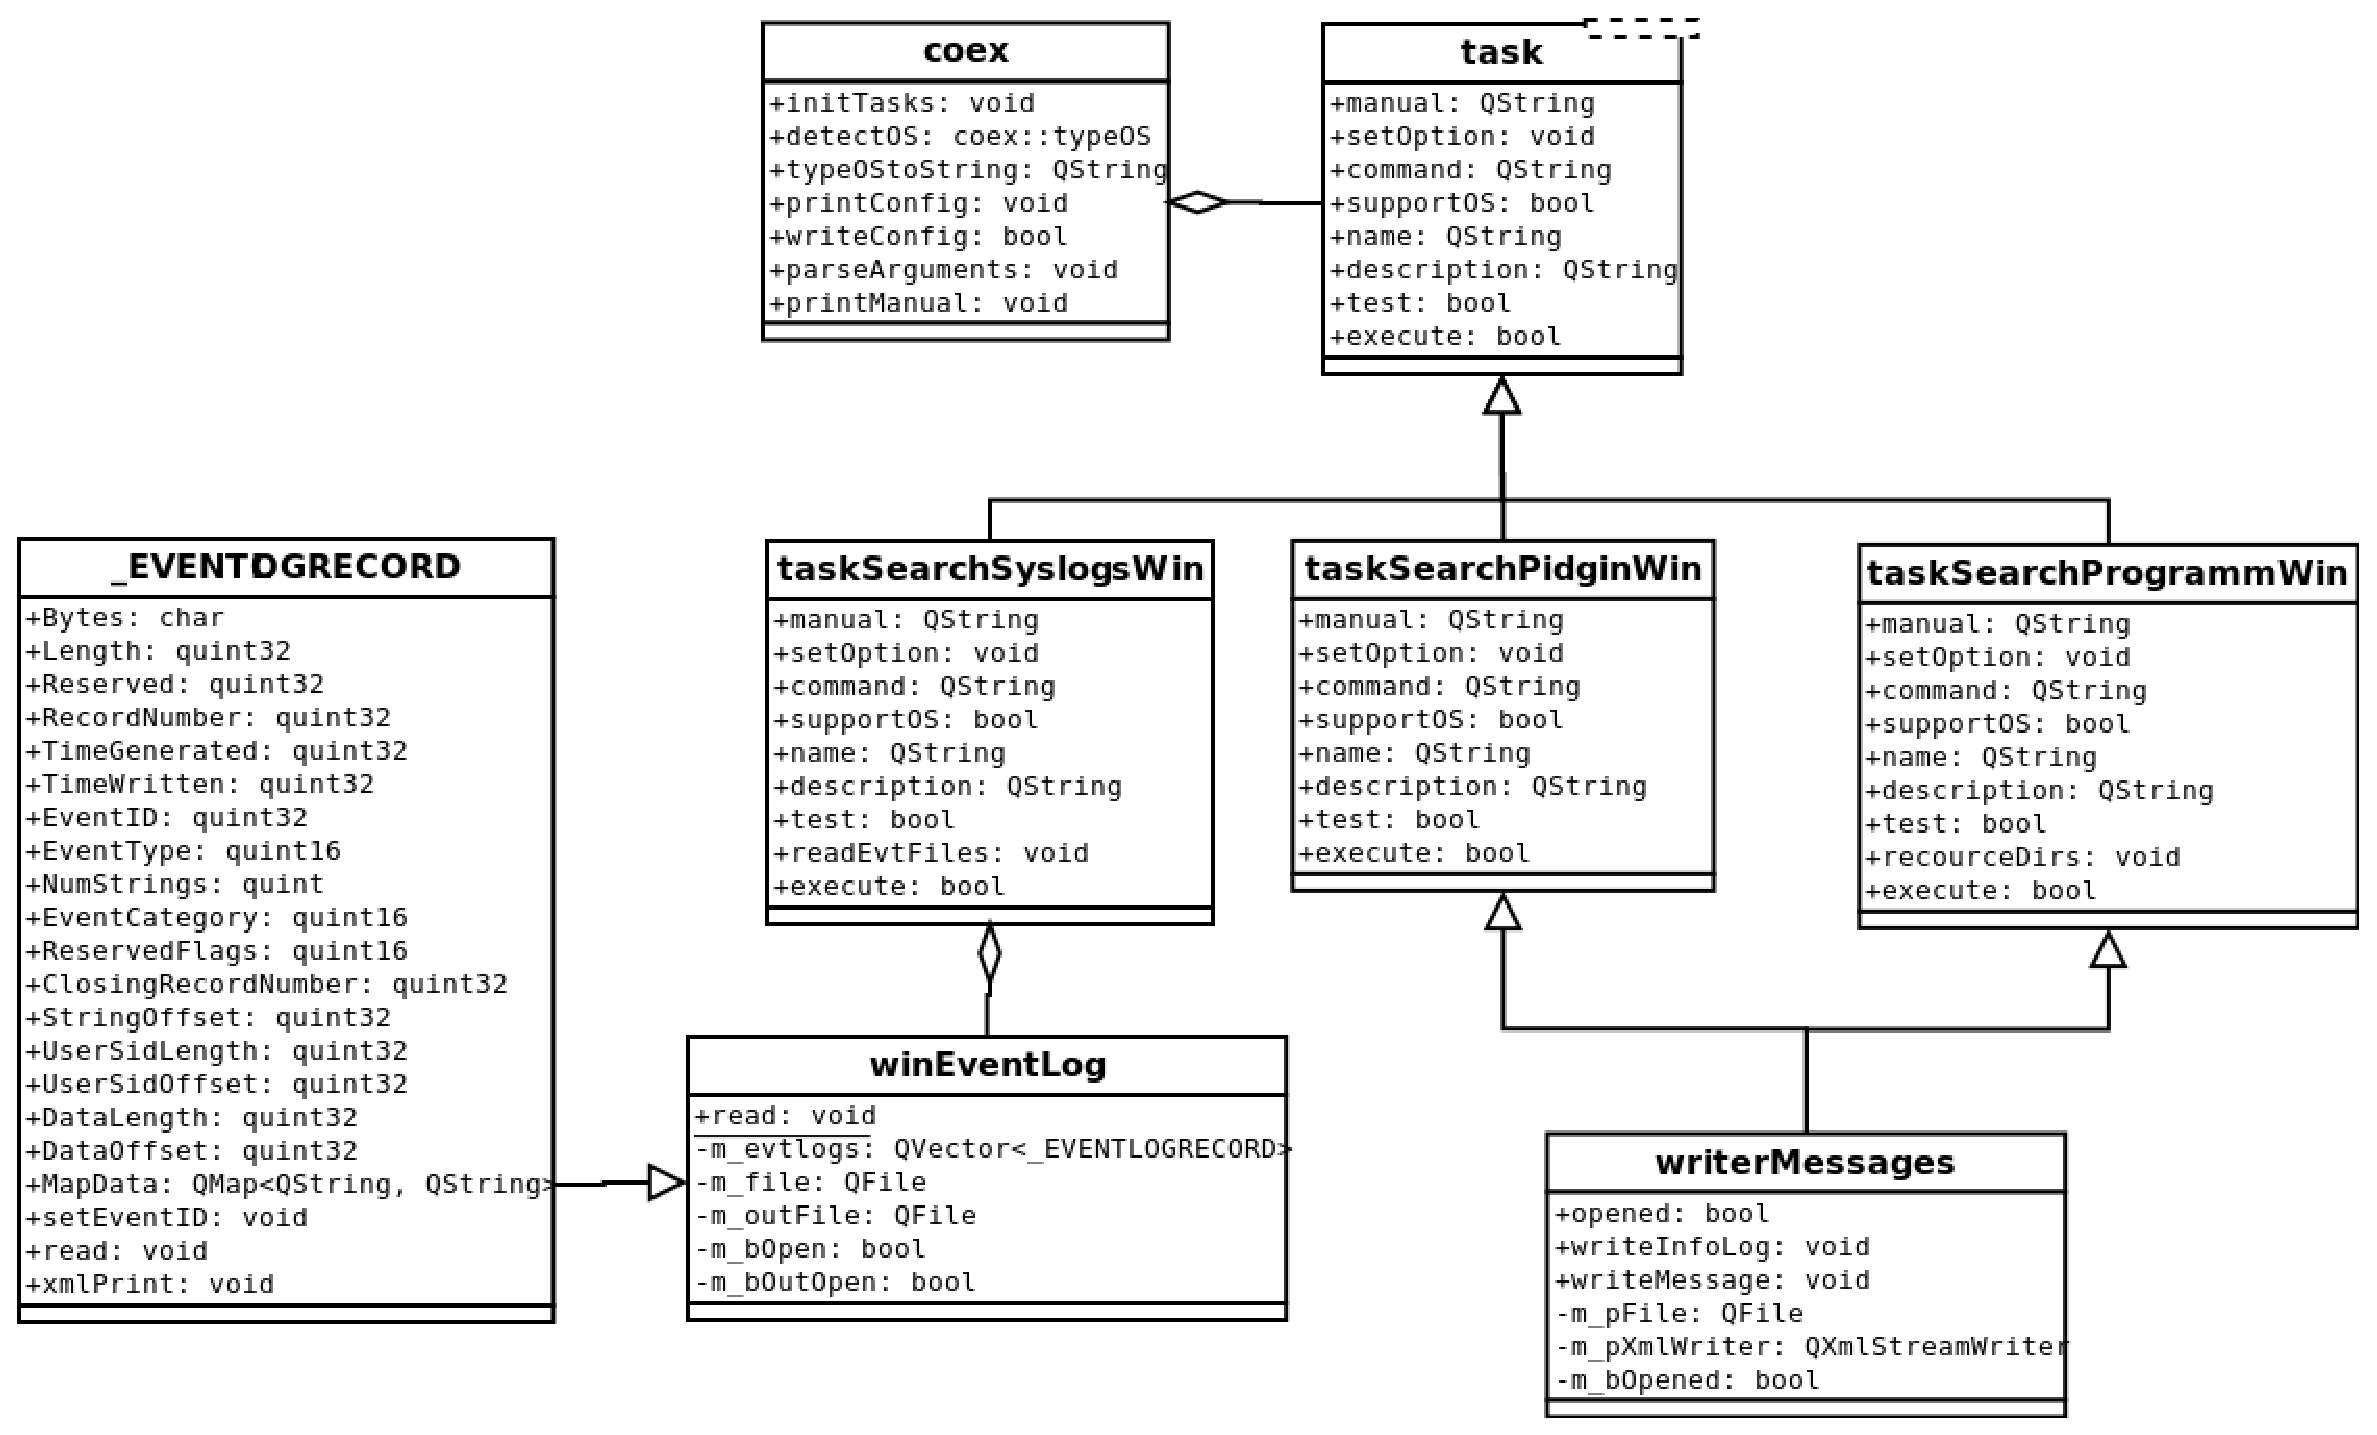
\includegraphics[width=0.9\linewidth]{UML}}
\caption{UML-диаграмма классов}
\label{UML:UML}
\end{figure}

Классы taskSearchSyslogsWin, taskSearchPidginWin и taskSearchSkypeWin - наследники от класса task являются тасками. Класс winEventLog и \_EVENTLOGRECORD предназначины для конвертации журнальных файлов операционной системы Windows XP, а класс writerMessages для преобразования истории переписки.

\subsubsection{Описание основных функций модуля системы}

Любой модуль системы является классом-наследником от некоторого абстрактного класса используемого как основу для всех модулей программы (шаблон проектирования Factory method). Модуль содержит в себе 8 методов и 3 атрибута:

QString manual() - возвращает справку о входных параметрах данного таска;

void setOption(QStringList list) - установка флагов для поданных на вход параметров;

QString command() - возвращает команду для инициализации такска вручную;

bool supportOS(const coex::typeOS \&os) - возвращает флаг указывающий на возможность использования данного таска для конкретной операционной системы;

QString name() - возвращает имя данного таска;

QString description() - возвращает краткое описание таска;

bool test() - предназначена для проверки работоспособности таска;

bool execute(const coex::config \&config) - запуск таска на выполнение;

QString m\_strName - хранит имя таска;

QString m\_strDescription - хранит описание таска;

bool m\_bDebug - флаг для параметра –debug.

\clearpage
